\chapter{知识图谱的数据模型---RDF\& OWL}\label{sec:RDFIntroduction}
\section{RDF数据三元组模型}\label{sec:RDFModel}
\indent
     从知识图谱数据组织的架构来看,可以把知识图谱的数据分为两个层次,一个是数据模型层,数据模型是按照本体论的思想,勾画出来的数据组织模式,数据模型可以展示数据的组织方式,数据之间的相互关系,创建动植物的数据模型,可以按照动植物的通用分类标准,使用七个主要级别:界、门、纲、目、科、属、种 。可以将动植物的数据按照这个模型进行组织。 a instance of classify 数据模型可以看作是元数据,依据数据模型,数据才能得到有效的组织。数据模型除了确定对象之间的分类,关系,还要明确对象的属性,针对不同的知识图谱,需要收集的数据的内容也不相同,内容范围由对象的属性确定。数据模型的分类,关系反映了数据之间的关系特征,数据模型的属性反映了数据的内在特征。\\
      \indent
     另一个就是具体数据层,具体数据是一条条的知识,它是依据数据模型组织起来的。我们可以把数据模型看作是骨架,把具体数据看作是肌肉,两部分共同组成了一个健壮的整体,就是我们的知识图谱。不同类型的知识图谱,组织数据的方式也有所不同,涉及到具体数据,具体数据的内容也有差别。比如对于一个人物来说,如果是历史知识图谱,可能人物数据的内容主要侧重于人物的生平,主要事迹,人物关系等等,如果是文学知识图谱,人物数据的内容则会主要侧重人物的主要作品,师承关系,作品流派等等。\\
     \indent
     RDF数据模型的核心包括资源(resource)、属性(property)、RDF陈述(RDF statement)等,最为核心的是三元组,资源-关系-资源,RDF数据还可以用图描述,而图也是由一系列的三元组构建而成。\\
     \indent
     资源,这里的资源可以是表示的事物也可以是抽象的概念,比如书(具体)、计算机(具体)、量子力学(抽象)等等。在RDF中,每个资源拥有一个统一的资源标识符(URI)表示,URI是一个用来标识资源的字符串,它是万维网体系结构的重要组成部分,我们常用的网址叫做统一资源定位符(URL)是URI 中的其中一种。\\
     \indent
     RDF允许引入不包含任何URI标示的资源,被称为空白节点或者匿名资源,用于标示一种存在变量,空白节点不能用URI来全局处理,所以为了区分不同的空白节点,RDF解析器一般会为每个空白节点分配一个系统生成的内部名。\\
     \indent
     属性是用来描述资源之间的关系,比如父子关系、包含关系等,RDF的属性同样可以使用URI来标示,这使得万维网环境下全局性的标示资源以及资源的联系称为可能。\\
     \indent
     陈述描述了某个资源特定属性及属性值,表达为(主语、谓语、宾语)的三元组结构,RDF图是一个由大量的RDF三元组构成的集合,可以用一个URI来标识一个RDF图,RDF三元组可以看做是“节点-边-节点”的结构,它和万维网的图结构(文档-超链接-文档)相吻合。本质上,RDF图是节点和边均带有标签的有向图结构。\\
     \indent
     RDF图是一个由RDF三元组构成的集合,可以用一个URI来标识这个RDF图,称为具名图。词汇表通常是在每个命名空间中的一组URI。RDF词汇表是一组以“http://www.w3.org/1999/02/22-rdf-syntax-nx\#”为XML命名空间的URI。\\
     \indent
     RDF的表示方法是指RDF数据是如何存储和传输的。目前RDF序列化的主要方式有RDF/XML,N-Triples,Turtle,RDFa,JSON-LD等。\\
     \indent
     RDF/XML,这仅仅是RDF表示有效的XML,由于可以解析和存储XML现有的工具过多,因此最初提出并使用它。RDF/XML可以通过任何RDF工具读取和写入,但RDF/XML冗长且难以读写,通常不是最好的序列化格式。\\
     \indent
     N-Triples是一个最基本的RDF序列化,它的特点主要是每行只存一个三元组以及分析速度非常快,因此Unix命令行工具可以轻松地对其进行操作。它也是高度压缩的,因此DBpedia等大型公共RDF资源通常以N-Triples形式发布数据。\\

    \begin{figure}[htb]
    \center{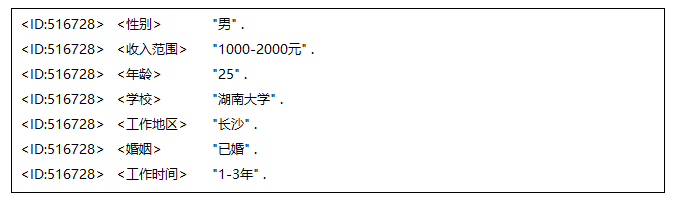
\includegraphics[width=12cm]  {./figures/part1/2.png}}
    \caption{\label{1} N-Triples实例}
    \end{figure}

    \indent
    现在写RDF,可能使用的是Turtle格式。Turtle比RDF / XML更紧凑,比N-Triples更可读,并且缺少Notation3的一阶逻辑扩展。此外,SPARQL查询语言以几乎完全相同的方式表达RDF查询。\\
    \subsection{RDF数据三元组模型}
    \indent
    任何事物都被表示成资源,通过URI表示出来;每个资源都有相关的属性及相应的属性值;每个资源还和其他资源有关系,多个资源相互链接就连成了一个语义网络图,每个资源及属性值,或者它与其他资源的一条关系都被称为一条知识,而这些属性和关系就能表示成三元组。\\
    \indent
    RDF的基本数据单元是一个三元组,可以表示为<主体,属性,客体>,这条三元组也可以称为是声明,这种方式主要是用来描述实体的相关属性。
    \begin{figure}[htb]
    \center{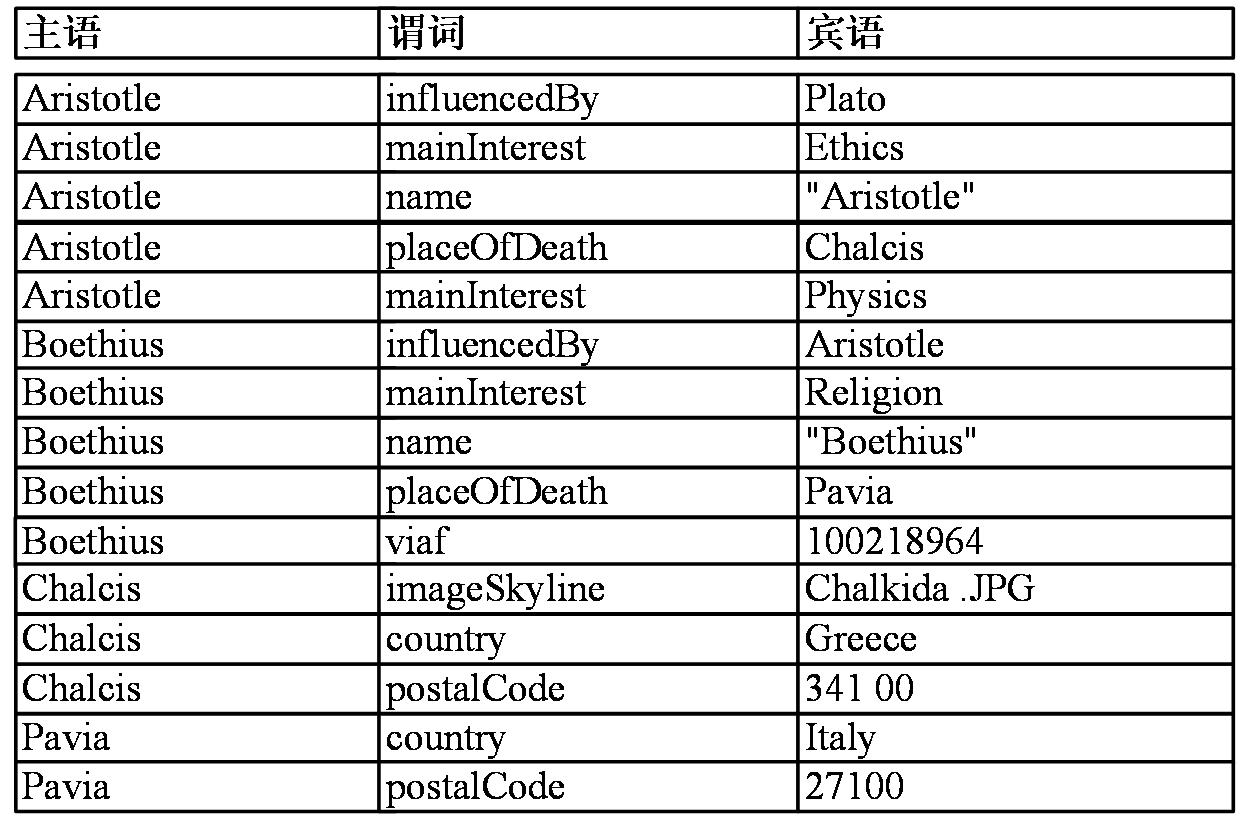
\includegraphics[width=10cm]  {./figures/part1/3.png}}
    \caption{\label{1} 三元组实例}
    \end{figure}

    \subsubsection{三元组}
    \indent
    三元组的顺序一般是按照<主语,谓语,宾语>的顺序编写,一个RDF三元组的三个组成部分:
    \begin{itemize}
    \item 主语,它是一个资源或者是一个空白节点。
    \item 谓语:它是一个资源标识符。
    \item 宾语:它可以是一个资源,也可以是一个文字节点,也可以是一个空白节点。
    \end{itemize}
    \indent
    三元组的主语和宾语就是RDF图中的一系列节点,一个谓词的资源标识符在同一张图里可能充当节点,也可能充当边,这二者都是有可能发生的。我们统一称呼资源标识符、文字节点、空白节点为RDF词语。资源标识符、文字节点、空白节点是唯一的并且可区分的,例如,http://example.org/作为一个字符串文字,既不等同于资源标识符http://example.org/,也不等同于一个http://example.org/标识的空白节点。\\
    \paragraph{资源标识符}
    \indent
    IRI(International Resource Identifier)称为国际化资源标识符。RDF抽象中的IRI必须是绝对的,并且可以包含片段标识符。\\
    IRIs的等效性:\\
    URIs和IRIs:URIs是IRI的一般化,并且URIs使用大部分的Unicode字符,每个绝对的URI和URL就是一个IRI,但并非所有的IRI都是一个URI;
    \paragraph{文字}
    文字就是为了表达字符串、数字、日期等一系列的值。一个RDF图中的一个文字节点由以下三个元素组成:
    \begin{itemize}
    \item 一个词汇形式:表示为一个Unicode字符串串;
    \item 一个数据类型IRI:作为一个IRI,识别并确定词汇形式如何映射到一个数据类型字面值
    \item 当且仅当所述的数据类型IRI是http://www.w3.org/1992/02/22-rdf-syntax-ns\#langString,这是一个非空的语义标记,语义标签必须是众所周知的。
    \end{itemize}
    \indent
    如果存在第三个元素,则文字是语言标记的字符串。语言标签的词汇可以转换为小写,语言标签的值空间也始终为小写。
    与文字相关的字面值:\\
    \begin{enumerate}
    \item 如果文字是一个语言标记的字符串,那么文字值就是有一个词汇形式和语言标记组成的对,按顺序排列。
    \item 如果文字的类型值IRI在已识别的数据类型IRI集合中,那么让d为数据类型IRI的指示对象。
    \subitem (1)如果文字的词汇形式是在d的词汇空间,则该文字值是施加的结果词法到值的映射的d到词汇形式。
    \subitem(2)否则,文字是错误的类型,没有文字值和该文字相关联。这种情况下就会产生语义的不一致,在语法上不合理,实现必须接受错误的文字并从中生成RDF图。实现可能会在遇到错误的文字时产生警告。
    \item 如果文字数据类型IRI不在已经识别的IRIs中,文字的字面值不会被规范化定义。
          文字术语等同性:当且仅当两个文字的词汇形式、两个数据类型IRI和语言标签,都逐个字符比较相等,两个文字就具有相同的文字值而不是相同的RDF 术语。

    \end{enumerate}
    \paragraph{空白节点}
    \indent
    空白节点不与文字节点和IRIs有任何交集,否则可能的空白节点集是任意的。RDF不参考任何空白节点的内部结构。空白节点标识符是一些具体的RDF语法或者RDF存储实现中使用的本地标识符。它们作用于文件或者是RDF仓库,但并不是空白节点的持久性或者可移植性的标识。空白节点并非RDF抽象语法的一部分,但是依赖于具体的的语法和具体的实现。因此,对于空白节点标识符的具体语法限制,也同样依取决于RDF的具体语法和具体的实现。在具体语法中处理空白节点标识符的实现需要注意不要从同一空白节点标识符的多次出现创建相同的空白节点,除非在语法支持的情况下。
    \paragraph{IRIs替换空白节点}
    \indent
    在RDF抽象语法中,空白节点没有任何标识符。由一些具体的语法引入的空白节点标识符具有局部作用,并且纯粹是一些序列化的工件。\\
    在需要更强识别的情况下,系统可以系统地利用一些IRI来替换RDF图中的部分空白节点。希望可以为空白节点挖掘一些新的、唯一的IRI,这样一来可以代替掉空白节点。\\
    如果Skolem IRI不会出现在任何地方,那么这种转换并没有明显改变RDF图的具体含义。然而它允许随后使用Skolem IRI的其他图形的可能性,但这对于空白节点不可能的。\\
    系统希望这样的方式使Skolem IRI成为可能,以便他们可以将IRI识别为仅用于替代空白节点。这允许系统在需要时将IRI映射回空白节点。\\
    \paragraph{图形比较}
    \indent
    如果两个图的节点集之间存在双射M的关系,则图G和G’之间是同构图的关系(他们具有相同的形式),比如:
    \begin{enumerate}
    \item M将空白节点映射到空白节点。
    \item M(lit)=lit对于所有的RDF文字节点是G的所有节点。
    \item M(iri)=iri对于所有的IRI标识符是G的所有节点。
    \item 三元组(s,p,o)是G的三元组,当且仅当三元组(M(s),p,M(o))是G’的三元组。
    \end{enumerate}
    \subsection{RDF数据模型}
    \indent
    RDF图由大量的三元组模型组成,其中RDF图中的顶点就代表一个资源,对应到三元组的主体或者客体;边就代表两个顶点之间的关系,对到三元组的谓词、属性。以下是一个简单的图模型实例:
    \begin{figure}[htb]
    \center{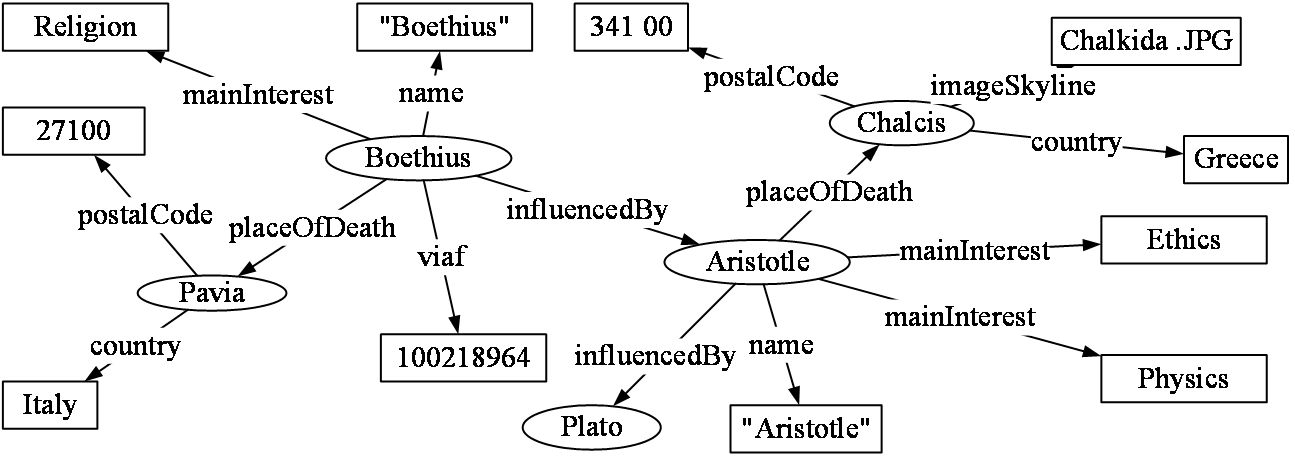
\includegraphics[width=10cm]  {./figures/part1/4.png}}
    \caption{\label{1} RDF图模型}
    \end{figure}
	
	
   \section{OWL简介}\label{sec:OWL}

    \indent
    OWL(Ontology Web Language)成为网络本体语言,旨在表示相关的事物,事务组与相关的事物之家丰富而复杂的知识,它属于一种计算逻辑语言,使得OWL中表达的知识可以被计算机利用,例如以验证知识的一致性和隐式知识明确。是基于DAML+OIL语言取长补短发展而来的,而DAML+OIL本身又是DAML和OIL 结合发展而来的,由W3C这个组织负责维护。\\
    \indent
    OWL Web本体语言是为那些需要处理信息内容的应用程序而设计的,而不仅仅是将信息呈现给人类。OWL通过提供额外的表达能力和形式化语义,使得Web内容的机器可解释性比XML、RDF和RDF Schema (RDF- s)所支持的更强。\\
    \indent
    OWL的主要作用是描述本体,本体就好比PPAP一种形式化的统一化的针对某一事物或概念的描述用来消除可能出现的歧义性同时增强可理解性。OWL包括三种相应的子语言,即OWL Lite、OWL DL、OWL Full。\\
    \indent
    OWL Lite是表达能力最弱的子语言。\\
    \indent
    OWL DL(Description Logic,描述逻辑)将可判定推理能力和较强表达能力作为首要目标,而忽略了对RDFS的兼容性。\\
    \indent
    OWL Full包含OWL的全部语言成分并取消了OWL DL中的限制,它将RDFS扩展为一个完备的本体语言,支持那些不需要可计算性保证(no computational guarantees)但需要最强表达能力和完全自由的RDFS用户。\\





    \begin{table}[h]
        \centering
        \begin{tabular}{|c|c|c|} %l(left)居左显示 r(right)居右显示 c居中显示
            \hline
            主语&谓语&宾语\\
            \hline
            冷藏胰岛素注射液&适用&昏迷\\
            \hline
            1型糖尿病性乳腺病&症状&不规则乳腺增生\\
            \hline
            1型糖尿病性视网膜病变&症状&眼痛\\
            \hline
            1型糖尿病性酮症&并发症&糖尿病\\
            \hline
            3个月以内孕妇&忌用&利福平片\\
            \hline
            Barrett食管&就诊于&内科\\
            \hline
            Fanconi综合征&症状&消瘦\\
            \hline
            Fanconi综合征&适用&花菜\\

            \hline
        \end{tabular}
        \caption{三元组实例}
    \end{table}




\section{常见的RDF知识图谱数据集合}\label{sec:RDFDatasets}

Linked Data

\begin{figure}[h]
\begin{center}
   \includegraphics[width=11cm]{./figures/part1/lod-cloud.pdf}
    \caption{关联数据}
   \label{fig:linkeddata}
\end{center}
\end{figure}


\subsection{常见中文知识图谱数据集}\label{sec:ChineseDatasets}
\textbf{PKUBase.}
PKUBase

\textbf{CN-DBpedia.}
CN-DBpedia\cite{DBLP:CNDBpedia} CN-DBpedia是由复旦大学知识工场实验室研发并维护的大规模通用领域结构化百科知识图谱数据集。CN-DBpedia前身是复旦大学GDM中文知识图谱,是国内最早推出的也是目前最大规模的开放百科中文知识图谱数据集。CN-DBpedia涵盖数千万实体和数亿级的关系,相关知识服务API累计调用量已达6亿次。
CN-DBpedia以通用的百科知识沉淀为主线,以垂直纵深领域图谱积累为支线,致力于为机器语义理解提供了丰富的背景知识,为实现机器语言认知提供必要支撑。

CN-DBpedia已经从百科领域延伸至法律、工商、金融、文娱、科技、军事、教育、医疗等十多个垂直领域,为各类行业智能化应用提供支撑性知识服务,目前已有近百家单位在使用。
CN-DBpedia具有体量巨大、质量精良、实时更新、丰富的API服务等特色。CN-DBpedia已经成为业界开放中文知识图谱的首选。基于CN-DBpedia的知识图谱构建与应用能力已经输出并应用在华为、小I机器人、中国电信、中国移动、同花顺等业界领军企业的产品与解决方案中。

CN-DBpedia提供全套API,并且免费开放使用。详细下载地址,可见http://kw.fudan.edu.cn/cndbpedia/intro/。



\subsection{常见外文知识图谱数据集}\label{sec:EnglishDatasets}
\textbf{DBpedia.}
DBpedia\cite{DBLP:DBpedia}
2007年开放。
目标是构建一个社区,通过社区成员定义和撰写准确的抽取模板,进而从维基百科中抽取结构信息,并将其发布到Web上。
社区通过人工的方式构建分类:
280个类别
覆盖约50%的维基百科实体


\textbf{YAGO.}
YAGO\cite{DBLP:YAGO,DBLP:YAGO2,DBLP:YAGO3}

\textbf{Freebase.}
Freebase\cite{url:Freebase}
2007年Metaweb公司发布。
2010年被Google收购。
大规模协同构建知识库。
从Wikipedia和其他数据源(如 IMDB、MusicBrainz)中导入知识
核心思想:
在Wikipedia中,人们编辑文章
在Freebase中,人们编辑结构化知识


